\chapter{Results}
\label{chap5}
\textit{This chapter presents the results of the experiments and evaluations conducted in this research. It provides a detailed analysis of the performance of MBRL algorithms with continue training and provide insights into the research questions posed at the beginning of this study.}

\section{Surrogate Model Performance}
To evaluate the surrogate model's performance, it is important to consider several critical metrics. These metrics serve as crucial indicators of how effectively the model approximates and forecasts the robot's behavior. Here, these metrics were elaborate without delving into details:
\begin{itemize}
    \item Average Steps before Failure: This metric assesses the model's capacity to predict the duration of a simulation run without encountering failure, serving as an indicator of sample efficiency.
    \item Validation RMSE and Validation Loss: This RMSE quantifies quantifies the disparity between the surrogate model's predictions and the actual values present in the validation dataset, as defined in Equation \ref{eq:RMSE}. Lower RMSE values are indicative of a higher degree of precision and accuracy in forecasting future states ($s_{t+1}$). Concurrently, the Validation Loss serves as an overarching measure of the model's performance on the validation dataset, underscoring the significance of minimizing this metric to enhance predictive capabilities, as defined in Equation \ref{eq:loss}.
    \item NRMSE: NRMSE provides a normalized measure of error,enabling comparisons of prediction accuracy across expert pattern datasets. It proves particularly valuable in evaluating the surrogate model's ability to predict sensor observations on the robot. The single step prediction NRMSE is calculated by Equation \ref{eq:NRMSE}, the long-term prediction NRMSE is calculated by Equation \ref{eq:NRMSET}.
    \item Correlation Coefficient (R): The R quantifies the linear relationship between simulated and predicted values, as specified in Equation \ref{eq:R}. A higher R signifies a more robust correlation, highlighting the model's proficiency in capturing underlying data trends and patterns.
\end{itemize}

\subsection{Model State-space Restriction}
The investigation commences with a focused exploration of state-space restriction within the surrogate model. The state-space, encompassing both observations and actions, is defined as $\mathbf{s}_t = [\mathbf{\theta}(t), \mathbf{v}(t), \mathbf{f}n(t), \mathbf{a}_{t-1}]$. Within this context, the boundaries of the action space play a pivotal role in shaping the behavior and adaptability of the soft quadruped robot. Specifically, our focus centers on two key components within the action space: the bending angle $\alpha_b$ and compression length $z_l$ of each diagonal leg pair. These parameters are fundamentally responsible for governing the robot's movements. Thus, a comprehensive understanding of the constraints associated with these parameters is essential for grasping how the robot behaves under various conditions and limitations.
\begin{figure}[htb]
    \centering
    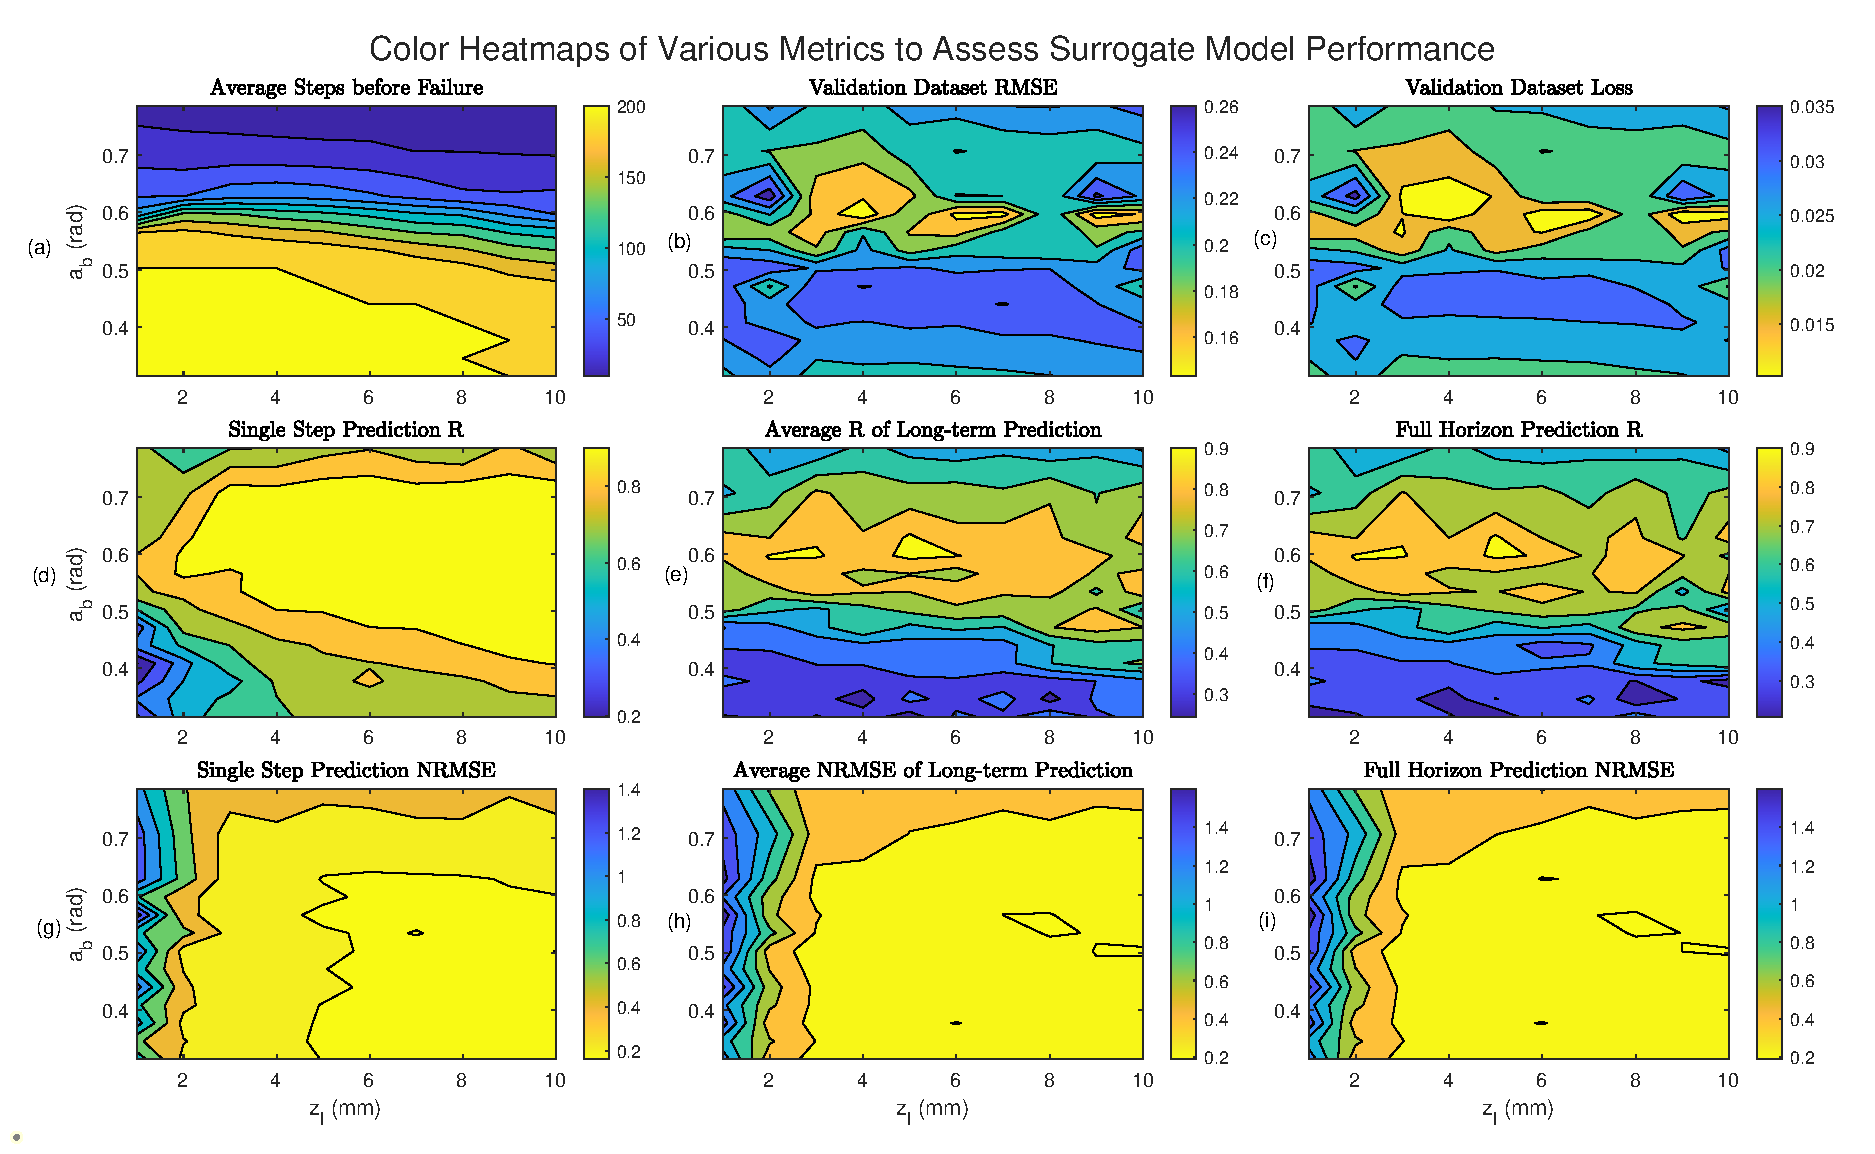
\includegraphics[width=\linewidth]{img/chap5/NN_heat.eps}
    \caption{Visualization of Performance Metrics Through Color Heat Map for Evaluating Trained Neural Networks. The metrics include: (a) Average Steps before Failure; (b) Root Mean Square Error (RMSE) on the Validation Dataset; (c) Loss on the Validation Dataset; (d) Single Step Prediction Coefficient R; (e) Average Coefficient R for Long-term Prediction; (f) Coefficient R for Full Horizon Prediction; (g) Normalized RMSE (NRMSE) for Single Step Prediction; (h) Average NRMSE for Long-term Prediction; (i) NRMSE for Full Horizon Prediction.}
    \label{fig:NN_heat}
\end{figure}

To address this aspect, a series of simulations involving random actions within a bounded action space were carried out. These simulations aimed to gather the necessary data required for training the surrogate model. Subsequently, the performance of the trained model was evaluated. To effectively assess the trained neural networks performance, a color heat map can be employed to provide a visual representation of various performance metrics, as shown in Figure \ref{fig:NN_heat}. Each metric is associated with a specific color scale, allowing for a quick and intuitive evaluation.

In Figure \ref{fig:NN_heat}(a), it is evident that reducing the lower restrictions within the action space leads to an increase in the average number of steps the system can take before encountering failure, indicating improved data efficiency due to reduced locomotion risk with smaller actions. In Figure \ref{fig:NN_heat}(c), all neural networks converge with a loss below 0.037 in the validation dataset, with minimal differences between them. In Figure \ref{fig:NN_heat}(b), validated in the same dataset, RMSE converges to a minimum level. Notably, better validation RMSE is achieved when $\alpha_b$ ranges from 0.55 to 0.7 radians and $z_l$ ranges from 3 to 9 millimeters, suggesting optimal model performance within these parameter ranges.

In assessing single-step predictions using various expert gait pattern datasets, the correlation coefficient (R) between predictions and ground truth was calculated, as depicted in Figure \ref{fig:NN_heat}(d). The results show consistently high accuracy when either the compression length ($z_l$) or the bending angle ($\alpha_b$) is high, or when both are elevated. This observation aligns with the expectation that for the robot to achieve higher speeds, it should exhibit more pronounced behaviors, which are characterized by larger values of these parameters. Consequently, the expert gait dataset used in this context emphasizes high values of $\alpha_b$ and $z_l$, resulting in smaller differences between predictions and ground truth, and consequently, lower values of R. A similar trend is observed when considering the for single-step predictions. Smaller NRMSE values are associated with high values of $z_l$ and $\alpha_b$, but interestingly, low $\alpha_b$ values also yield small NRMSE values. This implys that bending angle ($\alpha_b$) exerts a more significant influence on robot locomotion. These results are visually represented in Figure \ref{fig:NN_heat}(g). However, it is important to note that neither the NRMSE nor R reach their lowest points in the highest $\alpha_b$ region, suggesting poorer predictions when too small steps are taken before simulation failure, resulting in an insufficient amount of useful data.

For multi-step predictions on the same expert gait pattern datasets, the effects of $\alpha_b$ and $z_l$ are similar in single step prediction, but the models with low $\alpha_b$ values perform less effectively in predicting over longer time horizons, suggesting a lack of robust generality in these models. However, as shown in Figure \ref{fig:NN_heat}(e), the average correlation coefficient (R) for long-term predictions reveals that models with relatively high values of both $\alpha_b$ and $z_l$ struggle to predict states over extended horizons. TThis challenge could be attributed to the larger action space, which introduces more unpredictability and subsequently leads to reduced performance compared to models with lower $z_l$ values when trained on the same dataset size. This trend is also evident in the full horizon prediction R, as depicted in Figure \ref{fig:NN_heat}(f), where predictions at relatively high values of both $\alpha_b$ and $z_l$ deteriorate. In addition, the average NRMSE of long-term predictions exhibits a similar performance to what was observed in single-step predictions. Lower errors are associated with larger values of $\alpha_b$ and $z_l$, but NRMSE also decreases when $\alpha_b$ reaches its highest values. These results are presented in Figure \ref{fig:NN_heat}(h). Interestingly, performance remains consistent when $\alpha_b$ is smaller than 0.72 radians and $z_l$ is larger than 3 millimeters. Likewise, in the case of NRMSE for full horizon prediction, there is no significant change in performance, as indicated in Figure \ref{fig:NN_heat}(i).

Hence, the optimal action state restrictions can be identified as approximately $\alpha_b$ around 0.6 radians and $z_l$ around 6 millimeters. However, it's important to consider that these restrictions also impact MBRL training, as they limit the range of exploration within the robot's action space. So as larger space as possible is preferred, so that the second optimal restriction area come to our mind, where $\alpha_b$ is around 0.62 radian and $z_l$ is around 8 mm could be chosen for the restrictions for the state space at surrogate model and MBRL training.
\section{Model-based RL Training}
After the surrogate model determined in Section \ref{sec:NN_design}, we can continue to training of MBRL for optimal gait controls, which will be used as a gait controller in robot to navigate with learned optimal gait. 
\section{Model-based RL Performance}
\begin{longtable}{|p{1cm}|cccccccc|}
\hline
    \multicolumn{1}{|c|}{\multirow{2}{*}{Method}} &
      \multicolumn{8}{c|}{\begin{tabular}[c]{@{}c@{}}Desired walking\\  speed $v_x$ (m/s)\end{tabular}} \\ \cline{2-9} 
    \multicolumn{1}{|c|}{} &
      \multicolumn{1}{c|}{0.01} &
      \multicolumn{1}{c|}{0.1} &
      \multicolumn{1}{c|}{0.3} &
      \multicolumn{1}{c|}{0.5} &
      \multicolumn{1}{c|}{0.75} &
      \multicolumn{1}{c|}{1} &
      \multicolumn{1}{c|}{1.5} &
      3 \\ \hline
    \endfirsthead
    %
    \endhead
    %
    Model-based RL &
      \multicolumn{1}{c|}{\begin{tabular}[c]{@{}c@{}}Test 1:\\ Test 2:\\ Test 3:\end{tabular}} &
      \multicolumn{1}{c|}{\begin{tabular}[c]{@{}c@{}}Test 1:\\ Test 2:\\ Test 3:\end{tabular}} &
      \multicolumn{1}{c|}{\begin{tabular}[c]{@{}c@{}}Test 1:\\ Test 2:\\ Test 3:\end{tabular}} &
      \multicolumn{1}{c|}{\begin{tabular}[c]{@{}c@{}}Test 1:\\ Test 2:\\ Test 3:\end{tabular}} &
      \multicolumn{1}{c|}{\begin{tabular}[c]{@{}c@{}}Test 1:\\ Test 2:\\ Test 3:\end{tabular}} &
      \multicolumn{1}{c|}{\begin{tabular}[c]{@{}c@{}}Test 1:\\ Test 2:\\ Test 3:\end{tabular}} &
      \multicolumn{1}{c|}{\begin{tabular}[c]{@{}c@{}}Test 1:\\ Test 2:\\ Test 3:\end{tabular}} &
      \begin{tabular}[c]{@{}c@{}}Test 1:\\ Test 2:\\ Test 3:\end{tabular} \\ \hline
    Model-free RL &
      \multicolumn{1}{c|}{\begin{tabular}[c]{@{}c@{}}Test 1:\\ Test 2:\\ Test 3:\end{tabular}} &
      \multicolumn{1}{c|}{\begin{tabular}[c]{@{}c@{}}Test 1:\\ Test 2:\\ Test 3:\end{tabular}} &
      \multicolumn{1}{c|}{\begin{tabular}[c]{@{}c@{}}Test 1:\\ Test 2:\\ Test 3:\end{tabular}} &
      \multicolumn{1}{c|}{\begin{tabular}[c]{@{}c@{}}Test 1:\\ Test 2:\\ Test 3:\end{tabular}} &
      \multicolumn{1}{c|}{\begin{tabular}[c]{@{}c@{}}Test 1:\\ Test 2:\\ Test 3:\end{tabular}} &
      \multicolumn{1}{c|}{\begin{tabular}[c]{@{}c@{}}Test 1:\\ Test 2:\\ Test 3:\end{tabular}} &
      \multicolumn{1}{c|}{\begin{tabular}[c]{@{}c@{}}Test 1:\\ Test 2:\\ Test 3:\end{tabular}} &
      \begin{tabular}[c]{@{}c@{}}Test 1:\\ Test 2:\\ Test 3:\end{tabular} \\ \hline
    
    
      \caption{ANCOVA tests examples for research question 2}
      \label{tab:rq2test}
\end{longtable}
In order to examine the operational capacity and investigate the gait patterns of the soft robot, we applied the above RL setups to learn the walking motions with different speed references $v_{ref}$, where the training settings are identical in each experiment. During the training experiments, we observe that the training performance of the simulated robot is susceptible to the reference speed $v_{ref}$. With a higher target velocity, the agent is able to walk forward in fewer training episodes with a converged policy. On the other hand, with a smaller $v_{ref}$ as the target, the agent is prone to pitch forward and the episode is terminated. We start the training process with various random seeds, and the training has a higher failure rate with the agent stuck in the local minimal. Hence intuitively, we regard mastering the low-speed locomotion policy as a more difficult task for the agent.


\subsection{Continue Learning}
Owing to the good exploration capacity in the SAC algorithm, a converged agent can be retrained with the potential to adapt the policy for different tasks. Therefore, the converged policy that leads the robot to walk at MBRL can be reused as the initialized policy in the continued training with more accurate model.

To accelerate the training process, we pre-determine a working behavior $A^e = [\textbf{a}_{t0}^e, ..., \textbf{a}_T^e]$, which provides the robot with an initial steady gait. In particular, we let the RL agent imitate the examples from the human knowledge by applying $A^e$ in the first second of each episode. Samples collected from these pairs are stored in the replay buffer and used later for learning. By this means, we resort to the framework of imitate learning methods. Even though our designed state–action trajectory cannot guarantee optimality, the agent can still benefit from emulating the guided elementary movements, leading to fast online implementation. 


\section{Field Test}
